\documentclass{beamer}

\usetheme{default}
\usecolortheme{rose}
\usepackage{hyperref}
\newcommand{\ignore}[1]{}
\setbeamerfont{alerted text}{series=\itshape}

\title{Descriptive Statistics}

% A subtitle is optional and this may be deleted
\subtitle{STAT-UB.0001 Statistics for Business Control}

\author{Ningshan Zhang}
% - Give the names in the same order as the appear in the paper.
% - Use the \inst{?} command only if the authors have different
%   affiliation.

\institute[New York University] % (optional, but mostly needed)
{
  IOMS Department\\
  nzhang@stern.nyu.edu
}
\date{July 3, 2018}
\AtBeginSubsection[]
{
  \begin{frame}<beamer>{Outline}
    \tableofcontents[currentsection,currentsubsection]
  \end{frame}
}

% Let's get started
\begin{document}

%-------------------
\begin{frame}
  \titlepage
\end{frame}



% Section and subsections will appear in the presentation overview
% and table of contents.

%-------------------
\begin{frame}{Descriptive Statistics}
Descriptive Statistics
\begin{itemize}
\item Methods of organizing, summarizing and presenting numerical data in a convenient form.
\item Descriptive statistics are the foundation for any statistical analysis.
\item What factors should you consider when deciding the best way to present your data?
\end{itemize}
\end{frame}

%-------------------
\begin{frame}{Qualitative vs Quantitative Data}
\begin{block}{Qualitative: categorical}
Examples:
\begin{itemize}
\item Level of Education
\item Movie genre
\end{itemize}
\end{block}

\begin{block}{Quantitative: numerical}
Examples:
\begin{itemize}
\item Interest rates
\item Temperature
\end{itemize}
\end{block}
\end{frame}

\ignore{
%-------------------
\begin{frame}{Qualitative or Quantitative?}
\begin{itemize}
\item Year in school
\item Major
\item Type of cell phone you own
\item Tablet ownership
\item Number of caffeinated beverages you drink per day
\end{itemize}
\end{frame}
}

%-------------------
\begin{frame}{Qualitative Data}
In the study of qualitative data, one usually wants to compare the amount of participants in one group relative to another group.
\begin{itemize}
\item Frequency: Number of observations falling into a particular group.
\item Relative Frequency: Proportions of observations falling into a particular group.
\end{itemize}
These can be presented numerically (table) or graphically (bar chart or pie chart).
\end{frame}

%-------------------
\begin{frame}{Movies by MPAA Rating in 2012}
Frequency Table\footnote{\tiny{Source: \url{www.the-numbers.com}, Movie2012.mtw}}
\begin{center}
\begin{tabular}{ |c|c| } \hline
 Rating & Frequency  \\ \hline\hline
 G & 14   \\ \hline
 PG & 59   \\ \hline
 PG-13 & 140   \\ \hline
 R  & 210   \\ \hline
 NC-17 & 2   \\ \hline
 Not Rated & 36   \\ \hline
\textbf{Total}  & \textbf{461}  \\ \hline
\end{tabular}
\end{center}
\end{frame}

%-------------------
\begin{frame}{Movies by MPAA Rating in 2012}
Frequency Table
 $\rightarrow$ Relative Frequency Table 
 \vspace{\stretch{1}}
 
\begin{tabular}{ |c|c| } \hline
 Rating & Frequency  \\ \hline\hline
 G & 14   \\ \hline
 PG & 59   \\ \hline
 PG-13 & 140   \\ \hline
 R  & 210   \\ \hline
 NC-17 & 2   \\ \hline
 Not Rated & 36   \\ \hline
\textbf{Total}  & \textbf{461}  \\ \hline
\end{tabular}
\  $\rightarrow$ \ 
\begin{tabular}{ |c|c| } \hline
 Rating & Rel. Frequency  \\ \hline\hline
 G &    \\ \hline
 PG &    \\ \hline
 PG-13 &    \\ \hline
 R  &    \\ \hline
 NC-17 &    \\ \hline
 Not Rated &    \\ \hline
\textbf{Total}  & \textbf{100\%}  \\ \hline
\end{tabular}
\end{frame}




%-------------------
\begin{frame}{Movies by MPAA Rating in 2012}
Bar chart of Frequencies
 \vspace{\stretch{1}}
\begin{center}
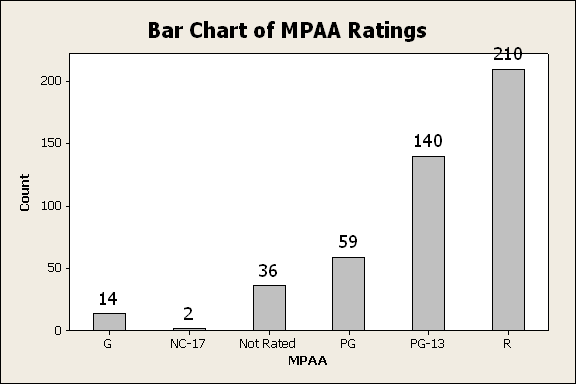
\includegraphics[width=0.8\textwidth]{figures/barchart.png}
\end{center}
\end{frame}

%-------------------
\begin{frame}{Movies by MPAA Rating in 2012}
Pie chart of Relative Frequencies
 \vspace{\stretch{1}}
\begin{center}
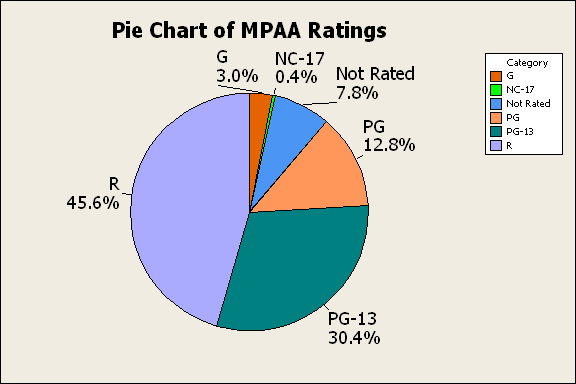
\includegraphics[width=0.8\textwidth]{figures/piechart.png}
\end{center}
\end{frame}

%-------------------
\begin{frame}{Charts Gone Bad}
According to the 2010 Cause Evolution Study\footnote{\tiny{\url{http://www.conecomm.com/2010-cone-communications-cause-evolution-study-pdf/}}},  `` ...  Consumers are willing to:''
\begin{center}
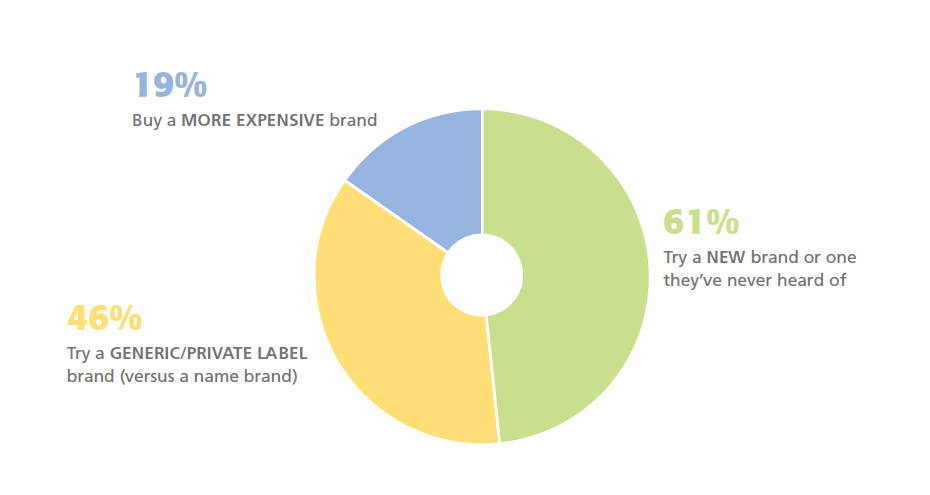
\includegraphics[width=0.8\textwidth]{figures/piechart_bad.png}
\end{center}
What is wrong with this chart?
\end{frame}


%-------------------
\begin{frame}{Quantitative Data}
In the study of quantitative data, one usually wants to find and display certain distributional properties.
\begin{block}{Numerical summaries}
\begin{itemize}
\item Measures of central tendency
\item Measures of variability
\item Identifying outliers
\end{itemize}
\end{block}
\begin{block}{Graphical summaries}
\begin{itemize}
\item Histograms
\item Boxplots
\item Time Series Plot
\end{itemize}
\end{block}
\end{frame}

%-------------------
\begin{frame}{Measures of Central Tendency: Mean vs Median}
\begin{block}{Mean}
The mean of a sample is the average of the observations:
$$\bar x = \dfrac{1}{n} \sum_{i=1}^n x_i
=\dfrac{1}{n} \left(x_1+x_2 + \dots+x_n\right). $$
\end{block}
\begin{block}{Median}
The median is the middle value in a \alert{sorted} dataset. 
\begin{itemize}
\item  When n is odd, take ``true'' middle value.
\item When n is even, take the average of the two middle values.
\end{itemize}
\end{block}
What is the mean and median of $\{6, 4, 19, 6, 12, 8, 13, 0\}$?
\end{frame}

\ignore{
%-------------------
\begin{frame}{Measures of Central Tendency: Mean vs Median}
\begin{block}{Mean}
\begin{itemize}
\item Useful when interested in long-term average outcomes, and have large dataset.
\item Sensitive to outliers.
\end{itemize}
\end{block}
\begin{block}{Median}
\begin{itemize}
\item Useful when ranking is important (e.g. SAT score).
\item Important in demographics.
\end{itemize}
\end{block}
\end{frame}
}
%-------------------
\begin{frame}{Measures of Central Tendency: Mean vs Median}
Comparing the mean and the median helps us detect skewness in the data. 
\vspace{\stretch{0.5}}

\begin{block}{(Nonparametric) Skewness}
\begin{itemize}
\item Positive/right skew:   mean - median $>0$ , mean is to the right of the median. 
\item Negative/left skew:   mean - median $<0$, mean is to the left of the median. 
\end {itemize}
\end{block}
\end{frame}


%-------------------
\begin{frame}{Positive/Right Skewed }
 Mean $>$ Median. Usually appears as a \alert{left}-leaning curve. Also called right-tailed since right tail is longer.
 \begin{center}
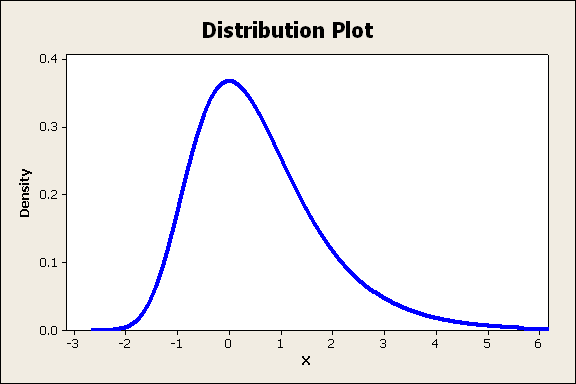
\includegraphics[width=0.8\textwidth]{figures/right_skew.png}
\end{center}
\end{frame}

%-------------------
\begin{frame}{Negative/Left Skewed }
 Mean $<$ Median. Usually appears as a \alert{right}-leaning curve. Also called left-tailed since left tail is longer.
 \begin{center}
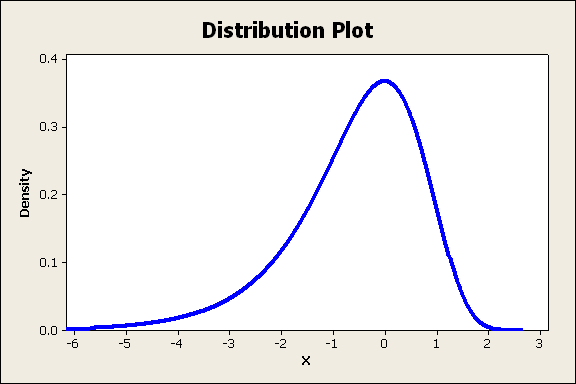
\includegraphics[width=0.8\textwidth]{figures/left_skew.png}
\end{center}
\end{frame}

%-------------------
\begin{frame}{Not Skewed or Symmetric}
 Mean $=$ Median. 
 \begin{center}
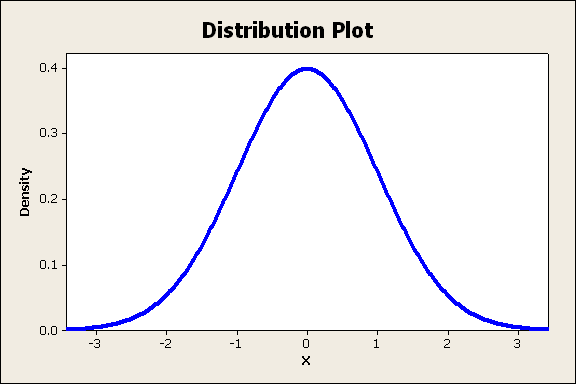
\includegraphics[width=0.8\textwidth]{figures/not_skew.png}
\end{center}
\end{frame}

%-------------------
\begin{frame}{Log Transformation}
The log transformation  usually can make highly skewed distributions, especially right skewed distributions less skewed. (But  not always.)

\begin{figure}
\caption{Left: Histogram of  $x$, the original data. Right: Histogram of $log(x)$.}
\begin{center}
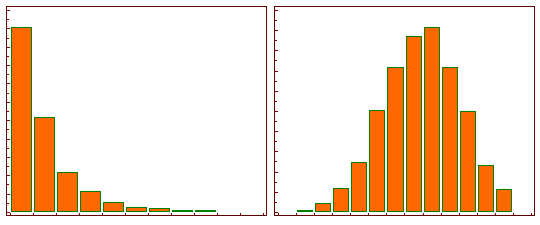
\includegraphics[width=0.8\textwidth]{figures/logtransformation}
\end{center}
\end{figure}

\let\thefootnote\relax\footnotetext{\tiny{* Plot from \url{https://www.medcalc.org/manual/log_transformation.php}}}


\end{frame}

%-------------------
\begin{frame}{Measures of Central Tendency: Mode}
\begin{block}{Mode}
The mode is the most common value in a data set.
\end{block}
Sample = $\{6, 4, 19, 6, 12, 8, 13, 0\}$. What is the mode? 
\vspace{\stretch{0.5}}

If the distribution is both symmetric and unimodal, then 
$$ \text{Mean = Median = Mode.}$$
\end{frame}

%-------------------
\begin{frame}{Measuring Variability}
Variability refers to the spread in the data. Common measures:


\begin{itemize}
\item Range, or Minimum \& Maximum.
\item Inter-Quartile.
\item Variance or Standard Deviation.
\end{itemize}
\end{frame}

%-------------------
\begin{frame}{Measuring Variability: Range}
The simplest measure of variability is the range of the data:
\begin{itemize}
\item Minimum = smallest value in a dataset.
\item Maximum = largest value in a dataset.
\item Range = Maximum - Minimum.
\end{itemize}
\vspace{\stretch{0.5}}

Example: $\{6, 4, 19, 6, 12, 8, 13, 0\}$.
\end{frame}

%-------------------
\begin{frame}{Measuring Variability: Inter-quartile Range
}
A more useful quantity is the inter-quartile range (IQR):
\begin{itemize}
\item 1st quartile = the $(n+1)/4$-th value in a sorted dataset (aka lower quartile, $Q_L$ , 25th percentile, $Q_1$).
\item 3rd quartile = the $3(n+1)/4$-th value in a sorted dataset (aka upper quartile, $Q_U$, 75th percentile, $Q_3$).
\item IQR = $Q_U - Q_L$.
\end{itemize}
\vspace{\stretch{0.5}}

Example: $\{6, 4, 19, 6, 12, 8, 13, 0\}$,
$Q_L = 4.5$, $Q_U = 12.75$.

\vspace{\stretch{0.5}}

Percentile: generalization of quartile, Qth percentile is the number such that Q\% of all observations are less to.
\end{frame}

%-------------------
\begin{frame}{Measuring Variability: Variance and Standard Deviation}
The most important measures of variability are the sample variance and the sample standard deviation.

\begin{itemize}
\item Sample Variance:
$$s^2 = \frac{1}{n-1}\sum_{i=1}^n (x_i - \bar x)^2
= \frac{1}{n-1} \sum_{i=1}^n (x_i^2 - n \bar x^2)$$
\item Sample standard deviation:
$$ s= \sqrt{s^2}$$
\end{itemize}
\vspace{\stretch{0.5}}

Example: $\{6, 4, 19, 6, 12, 8, 13, 0\}$.
\end{frame}



%-------------------
\begin{frame}{Z-score and Outliers}
\begin{block}{Z-score}
Z-score is the number of standard deviations the observation is away from the mean. Formally,
the z-score of $x$ is
$$ z = \frac{x - \bar x }{s},$$
where 
\begin{itemize}
\item $x$ is an observed value, 
\item $\bar x$ is the sample mean, 
\item  $s$ is the sample standard deviation.
\end{itemize}
\end{block}
\end{frame}


\begin{frame}{Z-score and Outliers}
Outliers are the observations with \alert{unusually} large or \alert{unusually} small values relative to the \alert{other values} in a data set.

\vspace{\stretch{0.5}}
In other words, outliers have large absolute z-scores.
\end{frame}


%-------------------
\begin{frame}{Identifying Outliers: Empirical Rule}
For roughly bell-shaped distributions,
\begin{itemize}
\item About 68\% of data will have z-scores in (-1,1), i.e. within the range $[\bar x - s, \bar x + s]$.
\item About 95\% of data will have z-scores in (-2,2), i.e. within the range  $[\bar x - 2 s, \bar x + 2s]$.

\item About 99.7\% of data will have z-scores in (-3,3), i.e. within the range  $[\bar x - 3 s, \bar x + 3s]$.

\end{itemize}
\end{frame}

%-------------------
\begin{frame}{Histograms}
Histograms provide a visual representation of the distribution of the data. Example\footnote{\tiny{Source: \url{www.the-numbers.com}, Movie2012.mtw}}:
\begin{center}
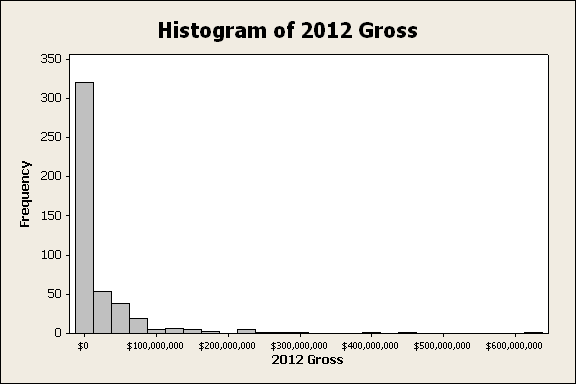
\includegraphics[width=0.8\textwidth]{figures/histogram.png}
\end{center}
\end{frame}


%-------------------
\begin{frame}{Histograms}
With a histogram, we can detect
\begin{itemize}
\item Skewness
\vspace{\stretch{0.2}}

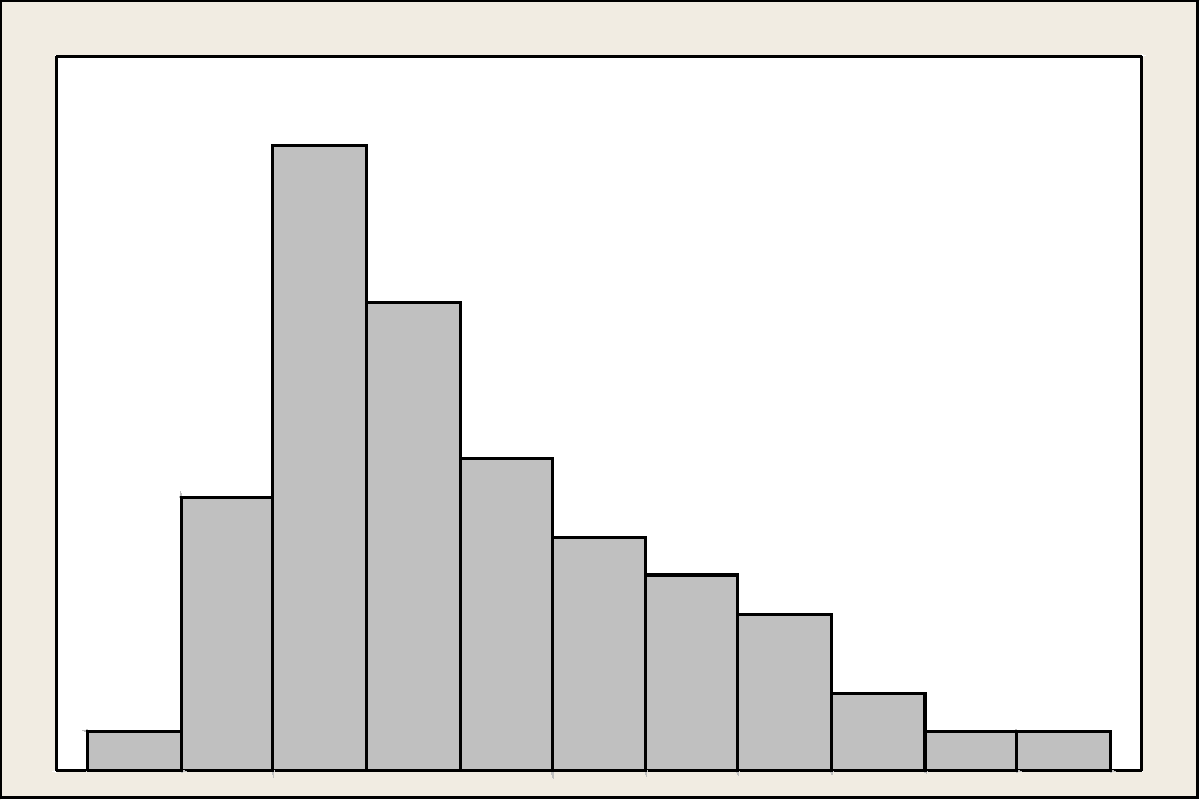
\includegraphics[width=0.25\textwidth]{figures/hist_skew}
\item Outliers
\vspace{\stretch{0.2}}

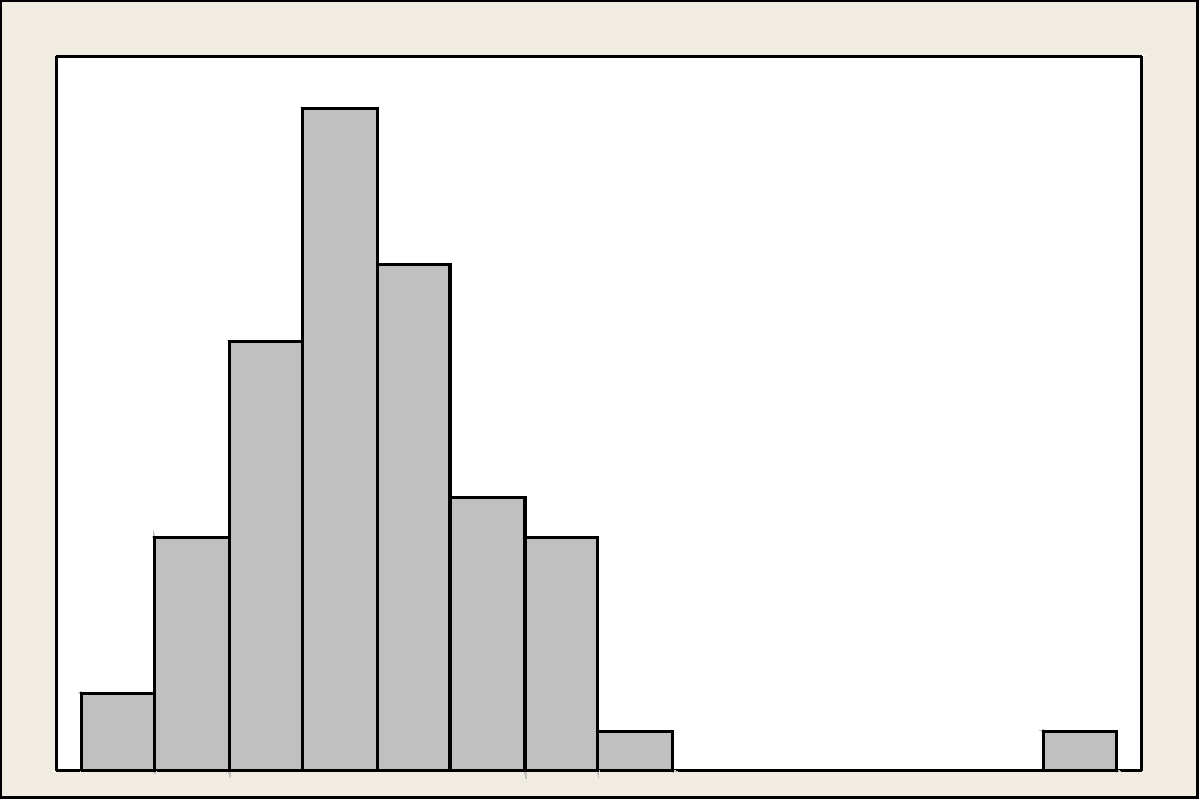
\includegraphics[width=0.25\textwidth]{figures/hist_outlier}
\item Bimodal distribution
\vspace{\stretch{0.2}}

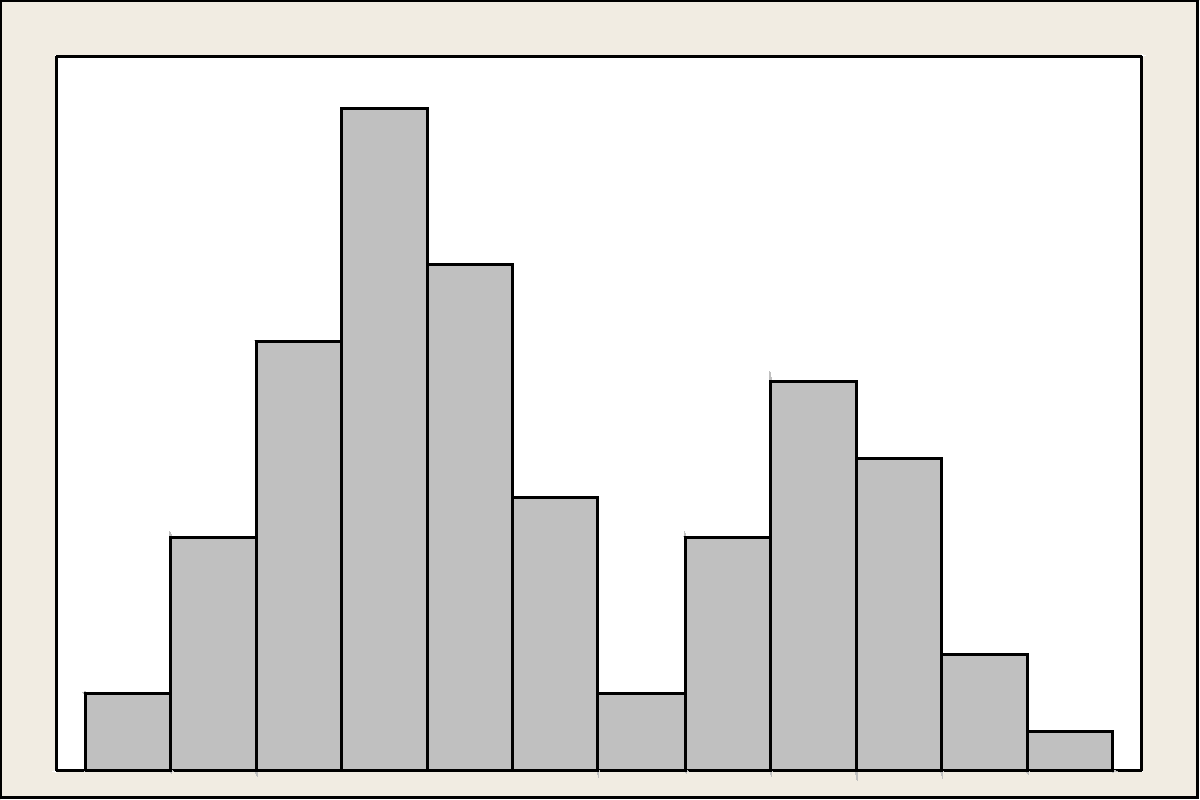
\includegraphics[width=0.25\textwidth]{figures/hist_bimodal}
\end{itemize}
\end{frame}

%-------------------
\begin{frame}{The Box-and-whisker plot}
Boxplots also provide a visual representation of the distribution of the data.
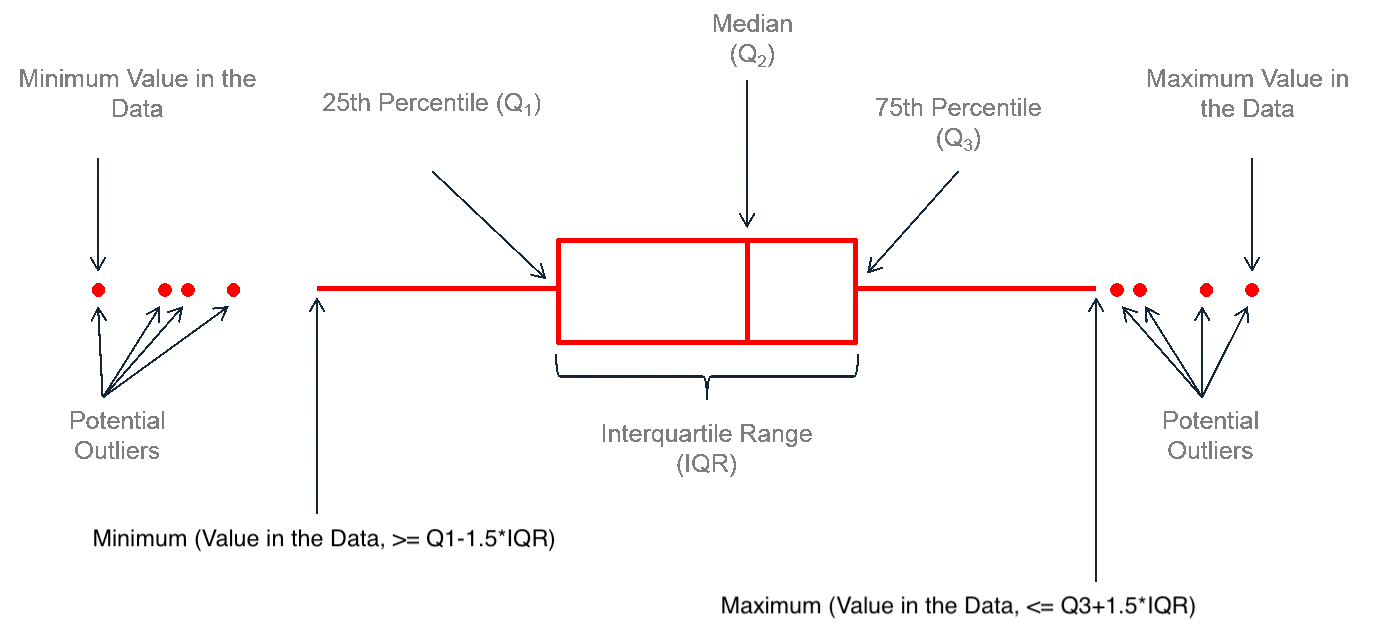
\includegraphics[width=1\textwidth]{figures/box_plot_copy.png}
\let\thefootnote\relax\footnotetext{\tiny{* Plot from \url{https://www.leansigmacorporation.com/box-plot-with-minitab/}}}
\end{frame}


%-------------------
\begin{frame}{Boxplots are excellent for comparing distributions}
\begin{figure}
\caption{Box plot of data from the Michelson�Morley experiment}
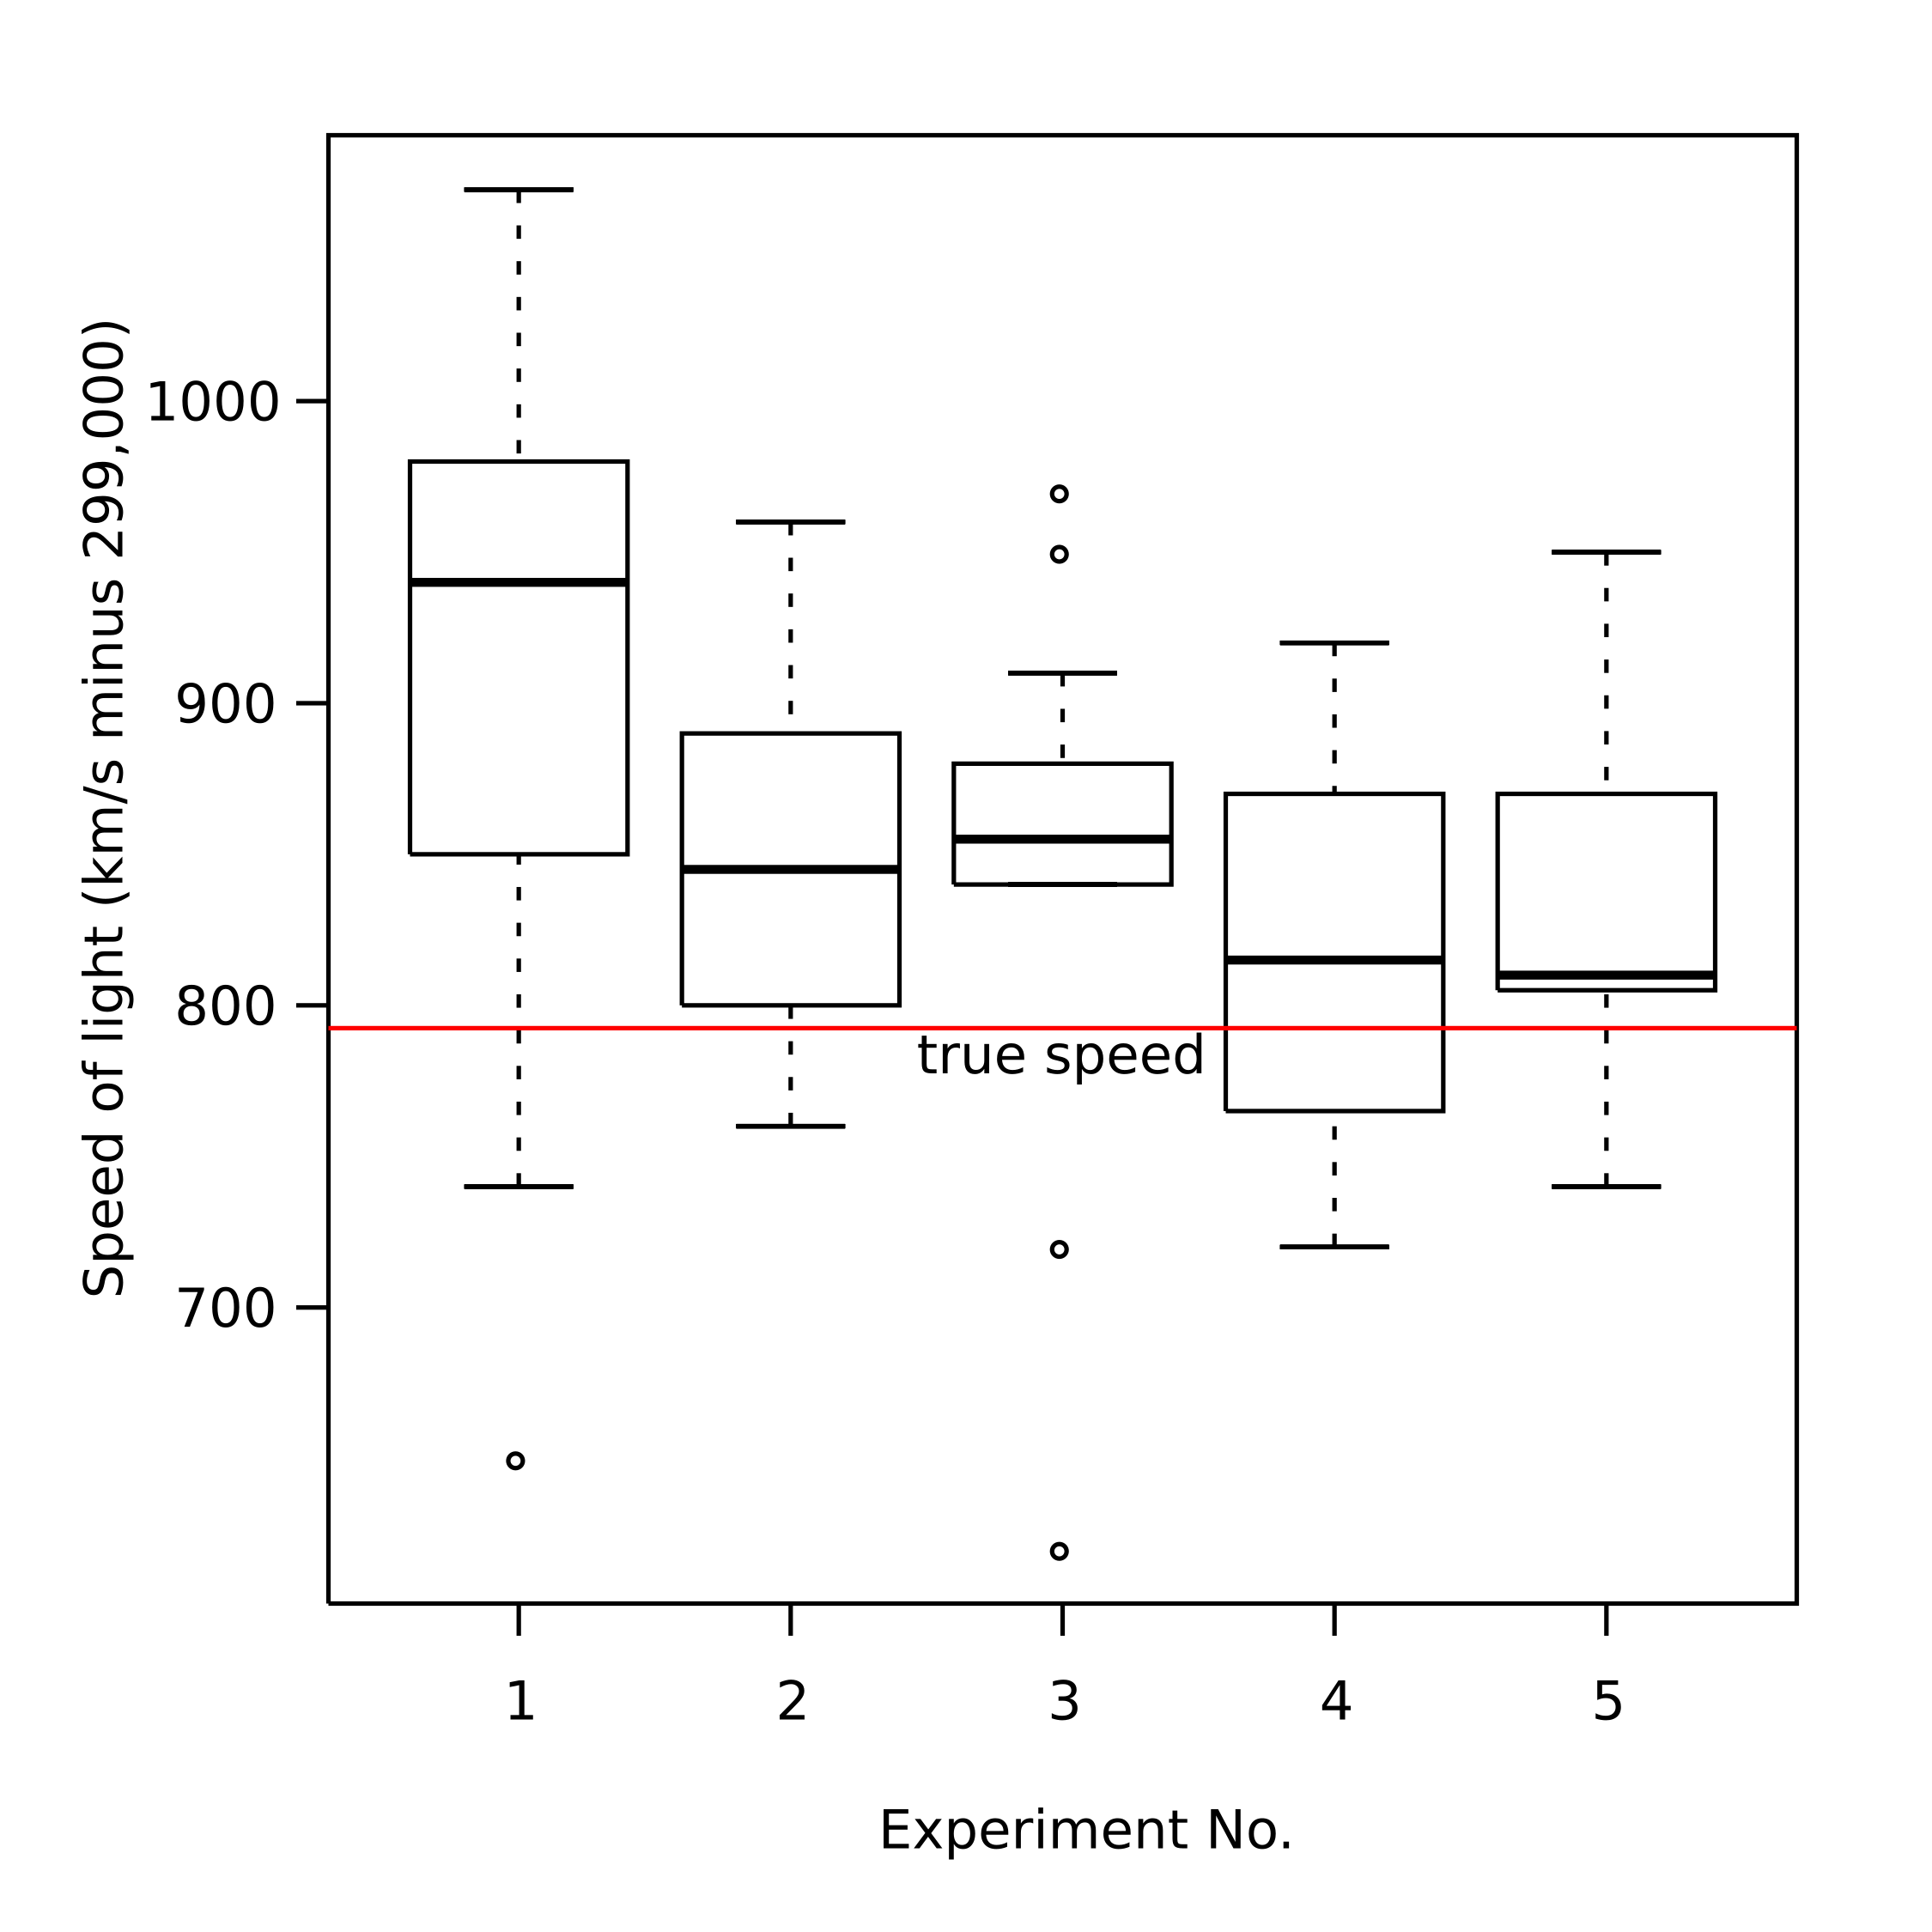
\includegraphics[width=0.6\textwidth]{figures/boxplot_compare.png}
\end{figure}
\let\thefootnote\relax\footnotetext{\tiny{* Plot from Wikipedia}}
\end{frame}


%-------------------
\begin{frame}{Identifying Outliers}
Two methods for identifying outliers:
\begin{itemize}
\item Z-score method
\begin{itemize}
\item Observations with z-scores outside $(-2,2)$ are outliers.
\item Stated differently, observations outside $(\bar x-2s,\bar x+2s)$ are outliers.
\end{itemize}
\item Boxplot method
\begin{itemize}
\item Observations outside $(Q_L-1.5* \text{IQR}, Q_U+1.5 *\text{IQR})$ are outliers. 
\item Observations outside $(Q_L-3*  \text{IQR}, Q_U+3*  \text{IQR})$ are serious outliers.
\end{itemize}
\end{itemize}

May produce different results.
\end{frame}

%-------------------
\begin{frame}{Time Series Plot}
Time series plots are useful when time sequencing is important.
\begin{figure}
\caption{Bitcoin Price from Jun 30, 2017 to Jun 30, 2018.}
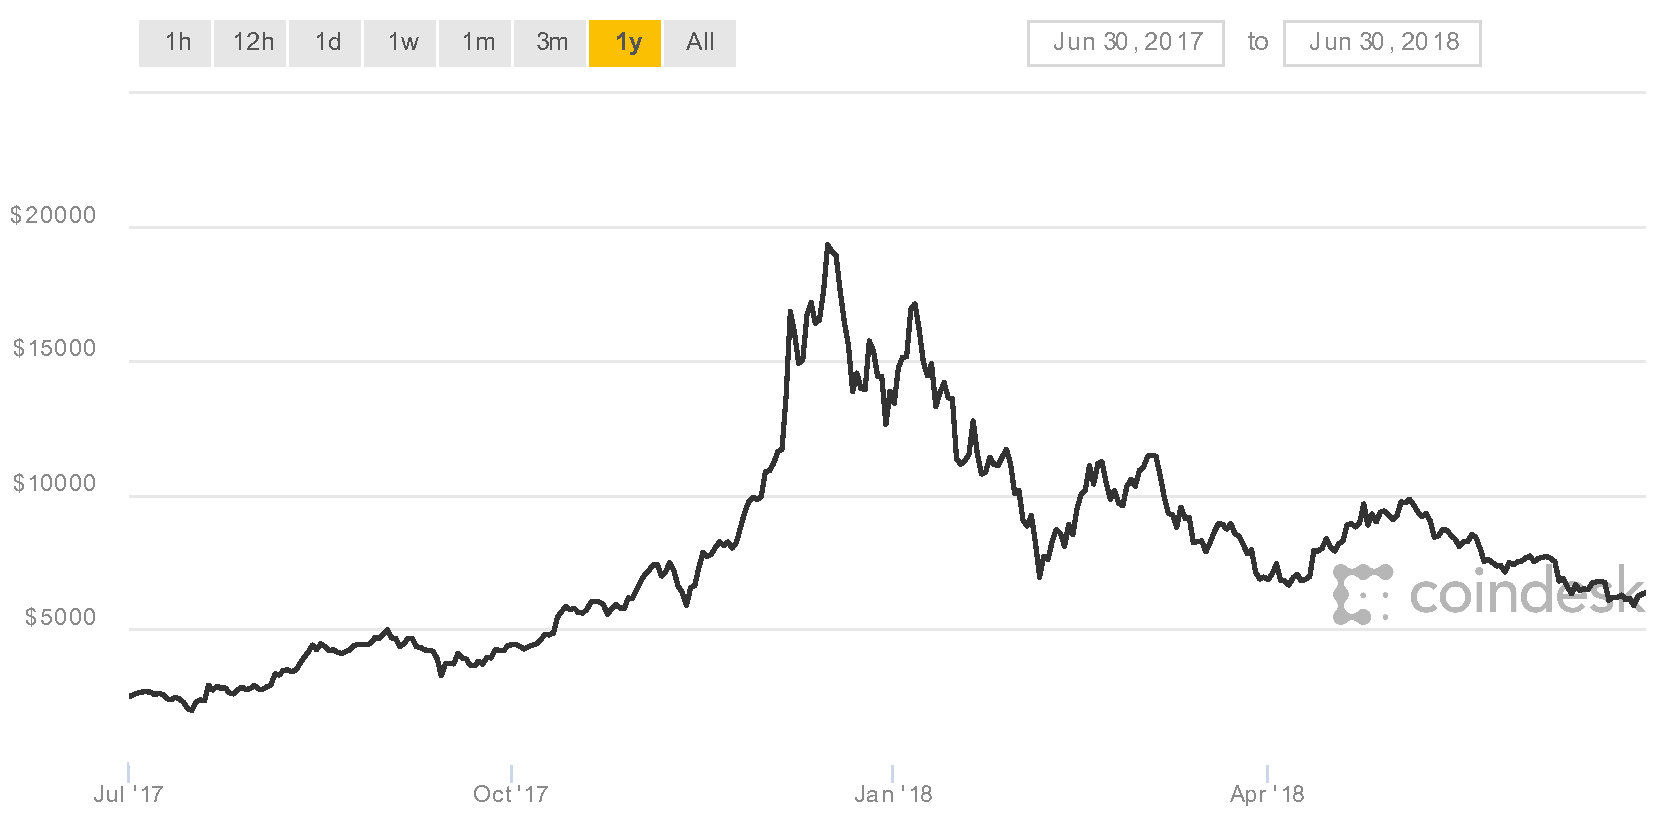
\includegraphics[width=1\textwidth]{figures/coindesk-bpi-chart}
\end{figure}
\let\thefootnote\relax\footnotetext{\tiny{* Plot from Coindesk.com}}
\end{frame}

%-------------------
\begin{frame}{Summary of Descriptive Statistics}
\begin{block}{Qualitative (Categorical)}
\begin{itemize}
\item Numerically: Frequency, Relative Frequency.
\item Graphically: Bar chart, Pie chart.
\end{itemize}
\end{block}
\begin{block}{Quantitative (Numerical)}
\begin{itemize}
\item Numerically
\begin{itemize}
\item Measures of central tendency  (mean, median, mode).
\item Measures of variability (range, IQR, standard deviation).
\item  Identifying outliers (z-scores, empirical rule).
\end{itemize} 
\item Graphically: Histogram, Box plot, Time series plot.
\end{itemize}
\end{block}

\end{frame}

\end{document}


